\section{Problema D - Estimación mediante diferencias progresivas de Newton}

Reproduzca el apartado anterior utilizando el método de las diferencias progresivas de Newton. Compare los resultados obtenidos y extraiga las conclusiones.


\subsection{Análisis}

\subsubsection{Teoría}

\paragraph{Definición}
El método de las diferencias progresivas de Newton es el siguiente.

Dado una serie de datos:

$$ S = \{ x_k, y_k \}^n $$

Se definen los polinomios base como: 

\begin{equation}
	n_k(x) = \prod_{j=0}^{k-1} (x - x_j) 
\end{equation}

con $n_0(x) = 1$.

El polinomio de interpolación es la combinación lineal de los polinomios base:

\begin{equation}
	N(x) = \sum_{k=0}^{n} [y_k] n_k(x)
\end{equation}

donde $[y_k]$ es la diferencia dividida.
\newpage

\subsection{Resolución}

\subsubsection{Programación}

\paragraph{Generación de polinomios} Los polinomios de orden 3 se generan con el código (muy similar al de lagrange):

\lstinputlisting[language=Python, firstline=4, lastline=37]{../../code/methods/newton.py}

Esto nos dará cinco polinomios, de los cuales solo usaremos dos, como en el siguiente snippet del código de los ejercicios.

\lstinputlisting[language=Python, firstline=16, lastline=16]{../../code/pecs/pec3/ex4.py}


\newpage 

\subsubsection{Polinomios generados vs muestras}

Una vez obtenidos los polinomios, pasamos a visualizarlos gráficamente.

\begin{figure}[H]
	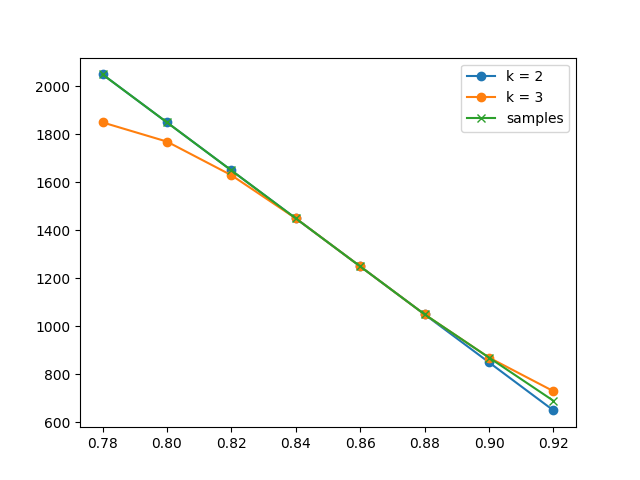
\includegraphics[width=\linewidth]{figures/figure4.png}
	\caption{Gráfica polinomios newton y la muestra}
	\label{fig:interp_newt}
\end{figure}



\newpage 
\paragraph{} 
Esto queda ilustrado en la siguiente figura, donde vemos la diferencia entre los dos polinomios. 

\begin{figure}[H]
	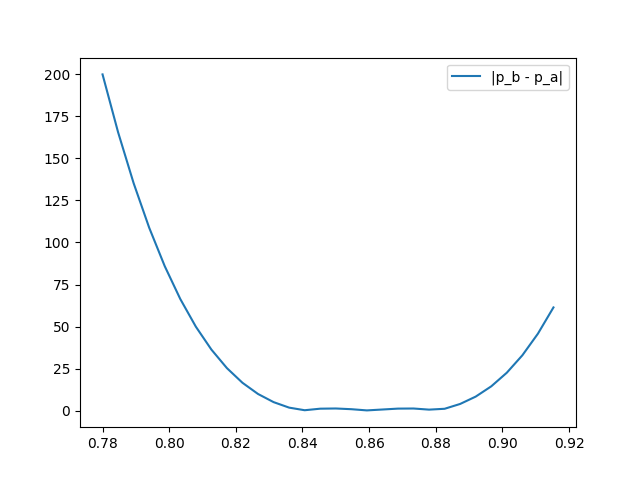
\includegraphics[width=\linewidth]{figures/figure5.png}
	\caption{Diferencia de los polinomios de newton}
	\label{fig:diff_interp_newt}
\end{figure}


\subsubsection{Resultados} 

Las edades interpoladas con los dos polinomios de newton ($k=2$, $k=3$) se ven en la siguiente tabla.

\begin{table}[htbp]
	\centering
	\csvreader[
	tabular=|c|c|c|,
	table head=\hline \textbf{\#} & \textbf{Age} \\\hline,
	late after last line=\\\hline,
	]{data/age03.csv}{}{\csvlinetotablerow}
\end{table}

\paragraph{Discusión} 
Los dos métodos para interpolar dan resultados idénticos en este contexto, por lo cual la elección de cual usar dependería del caso. Una ventaja del método de Newton es que si esperamos tener más muestras no habría que recalcular todo (con ligeras modificaciones el código podría reflejar esto).